\documentclass[11pt]{article}
\usepackage{amssymb}
\usepackage{listings}
\usepackage[margin=1in,footskip=0.25in]{geometry}
\usepackage{xcolor}
\usepackage{graphicx}
\usepackage{subfig}
\usepackage{float}

\definecolor{mygrey}{gray}{.96} % Light Grey
\definecolor{BrickRed}{RGB}{120,0,0}
\lstset{
	language=C++,              % choose the language of the code ("language=Verilog" is popular as well)
   tabsize=3,							  % sets the size of the tabs in spaces (1 Tab is replaced with 3 spaces)
	basicstyle=\footnotesize,               % the size of the fonts that are used for the code
	numbers=left,                   % where to put the line-numbers
	numberstyle=\footnotesize,              % the size of the fonts that are used for the line-numbers
	stepnumber=1,                   % the step between two line-numbers. If it's 1 each line will be numbered
	numbersep=5pt,                  % how far the line-numbers are from the code
	backgroundcolor=\color{mygrey}, % choose the background color. You must add \usepackage
	showspaces=false,              % show spaces adding particular underscores
	showstringspaces=false,        % underline spaces within strings
	showtabs=false,                % show tabs within strings adding particular underscores
	frame=single,	                 % adds a frame around the code
	tabsize=3,	                    % sets default tabsize to 2 spaces
	captionpos=b,                   % sets the caption-position to bottom
	breaklines=true,                % sets automatic line breaking
	breakatwhitespace=false,        % sets if automatic breaks should only happen at whitespace
	%escapeinside={\%*}{*)},        % if you want to add a comment within your code
	commentstyle=\color{BrickRed}   % sets the comment style
}
%Gummi|065|=)
\title{\Huge{\textbf{\underline{Monte Carlo Simulation: Assignment 1}}}}
\author{Yash Vanjani\\
		Roll No:140123046\\
		}
\date{21/01/2016}
\begin{document}
\maketitle
\Large{\textbf{\underline{Question 1}}}\\\\
\begin{center}$x_{i+1}=(ax_i+b)$ $mod$ $m$\end{center}
$$u_{i+1}=x_{i+1}/m$$
Generate the sequence of numbers $x_i$ for $a=6,b=0,\\m=11$ and $x_0$ ranging from 0 to 10. Also, generate the sequence of numbers $x_i$ for $a=3,b=0,m=11$, and $x_0$ranging from 0 to 10. Observe the sequence of numbers generated and observe the repetition of values. Tabulate these for each group of values. How many distinct values are appearing before repetitions? Which in your view are the best choices and why?\\\\
\Large{\textbf{\underline{Solution}}}\\\\
C++ Code:
\begin{lstlisting} [frame=single]
#include <iostream>
#include <fstream>


using namespace std;

int main()
{
	ofstream myfile;
	myfile.open("output.txt", ios::app);
	int i,j;
	int a,b,m;
	float x;
	float u;
	a=6;
	b=0;
	m=11;
	cout<<"For a=6, b=0, m=11:\n";
	myfile<<"For a=6, b=0, m=11:\n";

	for (i=0;i<11;i++)
	{
		cout<<"\nRandom x[i] for x[0]="<<i<<"\n";
		myfile<<"\nRandom x[i] for x[0]="<<i<<"\n";
		x=i;
		for(j=0;j<15;j++)
		{
			cout<<x<<" ";
			myfile<<x<<" ";
			x=((a*int(x))+b)%m;
		}
	}
	for(i=0;i<11;i++)
	{
		cout<<"\n";
		cout<<"Random u[i] for x[0]="<<i<<"\n";
		myfile<<"\n";
		myfile<<"Random u[i] for x[0]="<<i<<"\n";
		x=i;
		u=float(x/m);
		for(j=0;j<15;j++)
		{
			cout<<u<<" ";
			myfile<<u<<" ";
			x=((a*int(x))+b)%m;
			u=float(x/m);
		}
		cout<<"\n";
	}
	a=3;
	b=0;
	m=11;
	cout<<"\n\nFor a=3, b=0, m=11:\n";
	myfile<<"\n\nFor a=3, b=0, m=11:\n";
	for (i=0;i<11;i++)
	{
		cout<<"\nRandom x[i] for x[0]="<<i<<"\n";
		myfile<<"\nRandom x[i] for x[0]="<<i<<"\n";
		x=i;
		for(j=0;j<15;j++)
		{
			cout<<x<<" ";
			myfile<<x<<" ";
			x=((a*int(x))+b)%m;
		}
	}
	for(i=0;i<11;i++)
	{
		cout<<"\n";
		cout<<"Random u[i] for x[0]="<<i<<"\n";
		myfile<<"\n";
		myfile<<"Random u[i] for x[0]="<<i<<"\n";
		x=i;
		u=float(x/m);
		for(j=0;j<15;j++)
		{
			cout<<u<<" ";
			myfile<<u<<" ";
			x=((a*int(x))+b)%m;
			u=float(x/m);
		}
		cout<<"\n";
		myfile<<"\n";
	}
	myfile.close();
}

\end{lstlisting}
Output:
\begin{lstlisting}
For a=6, b=0, m=11:

Random x[i] for x[0]=0
0 0 0 0 0 0 0 0 0 0 0 0 0 0 0 
Random x[i] for x[0]=1
1 6 3 7 9 10 5 8 4 2 1 6 3 7 9 
Random x[i] for x[0]=2
2 1 6 3 7 9 10 5 8 4 2 1 6 3 7 
Random x[i] for x[0]=3
3 7 9 10 5 8 4 2 1 6 3 7 9 10 5 
Random x[i] for x[0]=4
4 2 1 6 3 7 9 10 5 8 4 2 1 6 3 
Random x[i] for x[0]=5
5 8 4 2 1 6 3 7 9 10 5 8 4 2 1 
Random x[i] for x[0]=6
6 3 7 9 10 5 8 4 2 1 6 3 7 9 10 
Random x[i] for x[0]=7
7 9 10 5 8 4 2 1 6 3 7 9 10 5 8 
Random x[i] for x[0]=8
8 4 2 1 6 3 7 9 10 5 8 4 2 1 6 
Random x[i] for x[0]=9
9 10 5 8 4 2 1 6 3 7 9 10 5 8 4 
Random x[i] for x[0]=10
10 5 8 4 2 1 6 3 7 9 10 5 8 4 2 
Random u[i] for x[0]=0
0 0 0 0 0 0 0 0 0 0 0 0 0 0 0 

Random u[i] for x[0]=1
0.0909091 0.545455 0.272727 0.636364 0.818182 0.909091 0.454545 0.727273 0.363636 0.181818 0.0909091 0.545455 0.272727 0.636364 0.818182 

Random u[i] for x[0]=2
0.181818 0.0909091 0.545455 0.272727 0.636364 0.818182 0.909091 0.454545 0.727273 0.363636 0.181818 0.0909091 0.545455 0.272727 0.636364 

Random u[i] for x[0]=3
0.272727 0.636364 0.818182 0.909091 0.454545 0.727273 0.363636 0.181818 0.0909091 0.545455 0.272727 0.636364 0.818182 0.909091 0.454545 

Random u[i] for x[0]=4
0.363636 0.181818 0.0909091 0.545455 0.272727 0.636364 0.818182 0.909091 0.454545 0.727273 0.363636 0.181818 0.0909091 0.545455 0.272727 

Random u[i] for x[0]=5
0.454545 0.727273 0.363636 0.181818 0.0909091 0.545455 0.272727 0.636364 0.818182 0.909091 0.454545 0.727273 0.363636 0.181818 0.0909091 

Random u[i] for x[0]=6
0.545455 0.272727 0.636364 0.818182 0.909091 0.454545 0.727273 0.363636 0.181818 0.0909091 0.545455 0.272727 0.636364 0.818182 0.909091 

Random u[i] for x[0]=7
0.636364 0.818182 0.909091 0.454545 0.727273 0.363636 0.181818 0.0909091 0.545455 0.272727 0.636364 0.818182 0.909091 0.454545 0.727273 

Random u[i] for x[0]=8
0.727273 0.363636 0.181818 0.0909091 0.545455 0.272727 0.636364 0.818182 0.909091 0.454545 0.727273 0.363636 0.181818 0.0909091 0.545455 

Random u[i] for x[0]=9
0.818182 0.909091 0.454545 0.727273 0.363636 0.181818 0.0909091 0.545455 0.272727 0.636364 0.818182 0.909091 0.454545 0.727273 0.363636 

Random u[i] for x[0]=10
0.909091 0.454545 0.727273 0.363636 0.181818 0.0909091 0.545455 0.272727 0.636364 0.818182 0.909091 0.454545 0.727273 0.363636 0.181818 


For a=3, b=0, m=11:

Random x[i] for x[0]=0
0 0 0 0 0 0 0 0 0 0 0 0 0 0 0 
Random x[i] for x[0]=1
1 3 9 5 4 1 3 9 5 4 1 3 9 5 4 
Random x[i] for x[0]=2
2 6 7 10 8 2 6 7 10 8 2 6 7 10 8 
Random x[i] for x[0]=3
3 9 5 4 1 3 9 5 4 1 3 9 5 4 1 
Random x[i] for x[0]=4
4 1 3 9 5 4 1 3 9 5 4 1 3 9 5 
Random x[i] for x[0]=5
5 4 1 3 9 5 4 1 3 9 5 4 1 3 9 
Random x[i] for x[0]=6
6 7 10 8 2 6 7 10 8 2 6 7 10 8 2 
Random x[i] for x[0]=7
7 10 8 2 6 7 10 8 2 6 7 10 8 2 6 
Random x[i] for x[0]=8
8 2 6 7 10 8 2 6 7 10 8 2 6 7 10 
Random x[i] for x[0]=9
9 5 4 1 3 9 5 4 1 3 9 5 4 1 3 
Random x[i] for x[0]=10
10 8 2 6 7 10 8 2 6 7 10 8 2 6 7 
Random u[i] for x[0]=0
0 0 0 0 0 0 0 0 0 0 0 0 0 0 0 

Random u[i] for x[0]=1
0.0909091 0.272727 0.818182 0.454545 0.363636 0.0909091 0.272727 0.818182 0.454545 0.363636 0.0909091 0.272727 0.818182 0.454545 0.363636 

Random u[i] for x[0]=2
0.181818 0.545455 0.636364 0.909091 0.727273 0.181818 0.545455 0.636364 0.909091 0.727273 0.181818 0.545455 0.636364 0.909091 0.727273 

Random u[i] for x[0]=3
0.272727 0.818182 0.454545 0.363636 0.0909091 0.272727 0.818182 0.454545 0.363636 0.0909091 0.272727 0.818182 0.454545 0.363636 0.0909091 

Random u[i] for x[0]=4
0.363636 0.0909091 0.272727 0.818182 0.454545 0.363636 0.0909091 0.272727 0.818182 0.454545 0.363636 0.0909091 0.272727 0.818182 0.454545 

Random u[i] for x[0]=5
0.454545 0.363636 0.0909091 0.272727 0.818182 0.454545 0.363636 0.0909091 0.272727 0.818182 0.454545 0.363636 0.0909091 0.272727 0.818182 

Random u[i] for x[0]=6
0.545455 0.636364 0.909091 0.727273 0.181818 0.545455 0.636364 0.909091 0.727273 0.181818 0.545455 0.636364 0.909091 0.727273 0.181818 

Random u[i] for x[0]=7
0.636364 0.909091 0.727273 0.181818 0.545455 0.636364 0.909091 0.727273 0.181818 0.545455 0.636364 0.909091 0.727273 0.181818 0.545455 

Random u[i] for x[0]=8
0.727273 0.181818 0.545455 0.636364 0.909091 0.727273 0.181818 0.545455 0.636364 0.909091 0.727273 0.181818 0.545455 0.636364 0.909091 

Random u[i] for x[0]=9
0.818182 0.454545 0.363636 0.0909091 0.272727 0.818182 0.454545 0.363636 0.0909091 0.272727 0.818182 0.454545 0.363636 0.0909091 0.272727 

Random u[i] for x[0]=10
0.909091 0.727273 0.181818 0.545455 0.636364 0.909091 0.727273 0.181818 0.545455 0.636364 0.909091 0.727273 0.181818 0.545455 0.636364 
\end{lstlisting}
\textbf{Answers}\\
\pagebreak
\\\Large{\textbf{\underline{Question 2}}\\\\
Generate a sequence $u_i$ with $m = 244944$, $a = 1597$ (take $x_0$ as per your choice).
Try to group the values in the ranges $0 - 0.05$, $0.05 - 0.10$, $0.10 - 0.15$, ... and see their
frequencies (i.e. the number of values falling in a group). For at least $5$ different values
of the number of values generated, tabulate the frequencies in each case, draw bar
diagrams of these data and put in your observations.  \\\\
\Large\textbf{{\underline{Solution}}}\\\\
C++ Code:
\begin{lstlisting}
#include <iostream>
#include <fstream>

using namespace std;

int main()
{
	ofstream myfile;
	myfile.open("output.txt", ios::app);
	
	int i,j,k,l;
	int a[2],b,m;
	float x[500000];
	int n[5];
	char filename[6];
	n[0]=1000;
	n[1]=500;
	n[2]=5000;
	n[3]=50000;
	n[4]=500000;
	float u[250000];
	int f[20];
	a[0]=1597;
	a[1]=51749;
	b=0;
	m=244944;
	char freq[20][100]={"0.00-0.05","0.05-0.10","0.10-0.15","0.15-0.20","0.20-0.25","0.25-0.30","0.30-0.35","0.35-0.40","0.40-0.45","0.45-0.50","0.50-0.55","0.55-0.60","0.60-0.65","0.65-0.70","0.70-0.75","0.75-0.80","0.80-0.85","0.85-0.90","0.90-0.95","0.95-1.00"};
	{
		myfile<<"For a="<<a[0]<<", b="<<b<<", m="<<m<<":\n";
		for (k=0;k<5;k++)
		{
			
			
			x[0]=12345;
			myfile<<"\nFor n="<<n[k];			
			u[0]=float(x[0]/m);
			for(j=0;j<n[k]-1;j++)
			{
				x[j+1]=((a[0]*int(x[j]))+b)%m;
				u[j+1]=float(x[j+1]/m);
			}
			myfile<<"\n";

			for(i=0;i<20;i++)
			{
				f[i]=0;
			}

			for(i=0;i<n[k];i++)
			{
				if(u[i]>=0 && u[i]<0.05)
					f[0]++;
				if(u[i]>=0.05 && u[i]<0.10)
					f[1]++;
				if(u[i]>=0.10 && u[i]<0.15)
					f[2]++;
				if(u[i]>=0.15 && u[i]<0.20)
					f[3]++;
				if(u[i]>=0.20 && u[i]<0.25)
					f[4]++;
				if(u[i]>=0.25 && u[i]<0.30)
					f[5]++;
				if(u[i]>=0.30 && u[i]<0.35)
					f[6]++;
				if(u[i]>=0.35 && u[i]<0.40)
					f[7]++;
				if(u[i]>=0.40 && u[i]<0.45)
					f[8]++;
				if(u[i]>=0.45 && u[i]<0.50)
					f[9]++;
				if(u[i]>=0.50 && u[i]<0.55)
					f[10]++;
				if(u[i]>=0.55 && u[i]<0.60)
					f[11]++;
				if(u[i]>=0.60 && u[i]<0.65)
					f[12]++;
				if(u[i]>=0.65 && u[i]<0.70)
					f[13]++;
				if(u[i]>=0.70 && u[i]<0.75)
					f[14]++;
				if(u[i]>=0.75 && u[i]<0.80)
					f[15]++;
				if(u[i]>=0.80 && u[i]<0.85)
					f[16]++;
				if(u[i]>=0.85 && u[i]<0.90)
					f[17]++;
				if(u[i]>=0.90 && u[i]<0.95)
					f[18]++;
				if(u[i]>=0.95 && u[i]<=1)
					f[19]++;
			}

			for(i=0;i<20;i++)
			{
				myfile <<i<<"	"<<freq[i]<<"	"<<f[i]<<"\n";
			}
			myfile<<"\n";
		}
	}
	myfile.close();		
}
\end{lstlisting}
Output:
\begin{lstlisting}
For a=1597, b=0, m=244944:

For n=1000
0	0.00-0.05	48
1	0.05-0.10	53
2	0.10-0.15	49
3	0.15-0.20	50
4	0.20-0.25	50
5	0.25-0.30	48
6	0.30-0.35	50
7	0.35-0.40	48
8	0.40-0.45	50
9	0.45-0.50	53
10	0.50-0.55	48
11	0.55-0.60	50
12	0.60-0.65	49
13	0.65-0.70	51
14	0.70-0.75	51
15	0.75-0.80	51
16	0.80-0.85	49
17	0.85-0.90	49
18	0.90-0.95	51
19	0.95-1.00	52


For n=500
0	0.00-0.05	26
1	0.05-0.10	25
2	0.10-0.15	26
3	0.15-0.20	28
4	0.20-0.25	18
5	0.25-0.30	24
6	0.30-0.35	29
7	0.35-0.40	22
8	0.40-0.45	24
9	0.45-0.50	25
10	0.50-0.55	22
11	0.55-0.60	28
12	0.60-0.65	24
13	0.65-0.70	21
14	0.70-0.75	32
15	0.75-0.80	27
16	0.80-0.85	20
17	0.85-0.90	26
18	0.90-0.95	26
19	0.95-1.00	27


For n=5000
0	0.00-0.05	248
1	0.05-0.10	254
2	0.10-0.15	247
3	0.15-0.20	251
4	0.20-0.25	250
5	0.25-0.30	246
6	0.30-0.35	252
7	0.35-0.40	247
8	0.40-0.45	251
9	0.45-0.50	256
10	0.50-0.55	245
11	0.55-0.60	248
12	0.60-0.65	246
13	0.65-0.70	252
14	0.70-0.75	253
15	0.75-0.80	247
16	0.80-0.85	250
17	0.85-0.90	251
18	0.90-0.95	256
19	0.95-1.00	250


For n=50000
0	0.00-0.05	2469
1	0.05-0.10	2521
2	0.10-0.15	2471
3	0.15-0.20	2525
4	0.20-0.25	2515
5	0.25-0.30	2467
6	0.30-0.35	2525
7	0.35-0.40	2468
8	0.40-0.45	2520
9	0.45-0.50	2518
10	0.50-0.55	2468
11	0.55-0.60	2522
12	0.60-0.65	2468
13	0.65-0.70	2517
14	0.70-0.75	2530
15	0.75-0.80	2470
16	0.80-0.85	2516
17	0.85-0.90	2471
18	0.90-0.95	2523
19	0.95-1.00	2516


For n=500000
0	0.00-0.05	24690
1	0.05-0.10	25205
2	0.10-0.15	24693
3	0.15-0.20	25208
4	0.20-0.25	25201
5	0.25-0.30	24691
6	0.30-0.35	25212
7	0.35-0.40	24692
8	0.40-0.45	25204
9	0.45-0.50	25205
10	0.50-0.55	24691
11	0.55-0.60	25204
12	0.60-0.65	24690
13	0.65-0.70	25201
14	0.70-0.75	25216
15	0.75-0.80	24692
16	0.80-0.85	25200
17	0.85-0.90	24693
18	0.90-0.95	25210
19	0.95-1.00	25202

\end{lstlisting}
Plots:\\\\
\begin{figure}[H]
	\centering
	\subfloat[$n=500$]{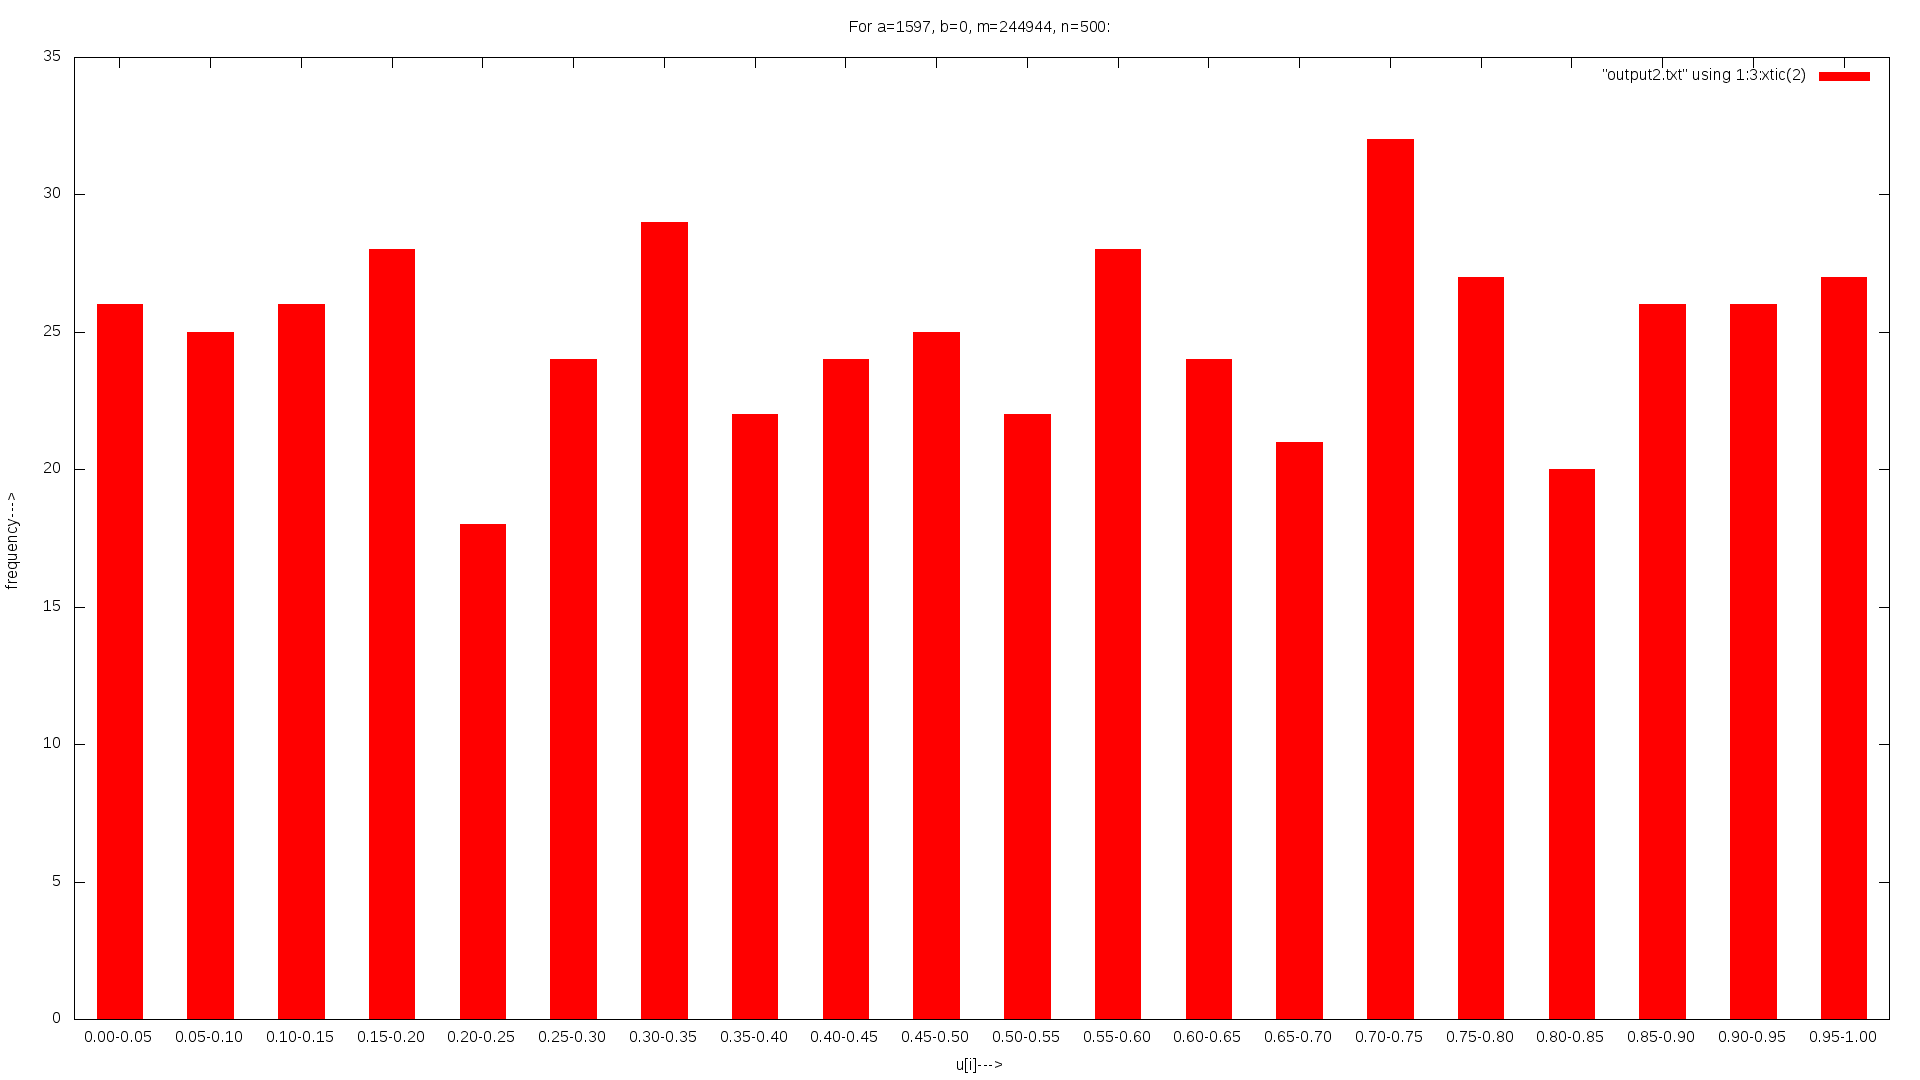
\includegraphics[width=0.5\textwidth]{plot2.png}}
	\subfloat[$n=1000$]{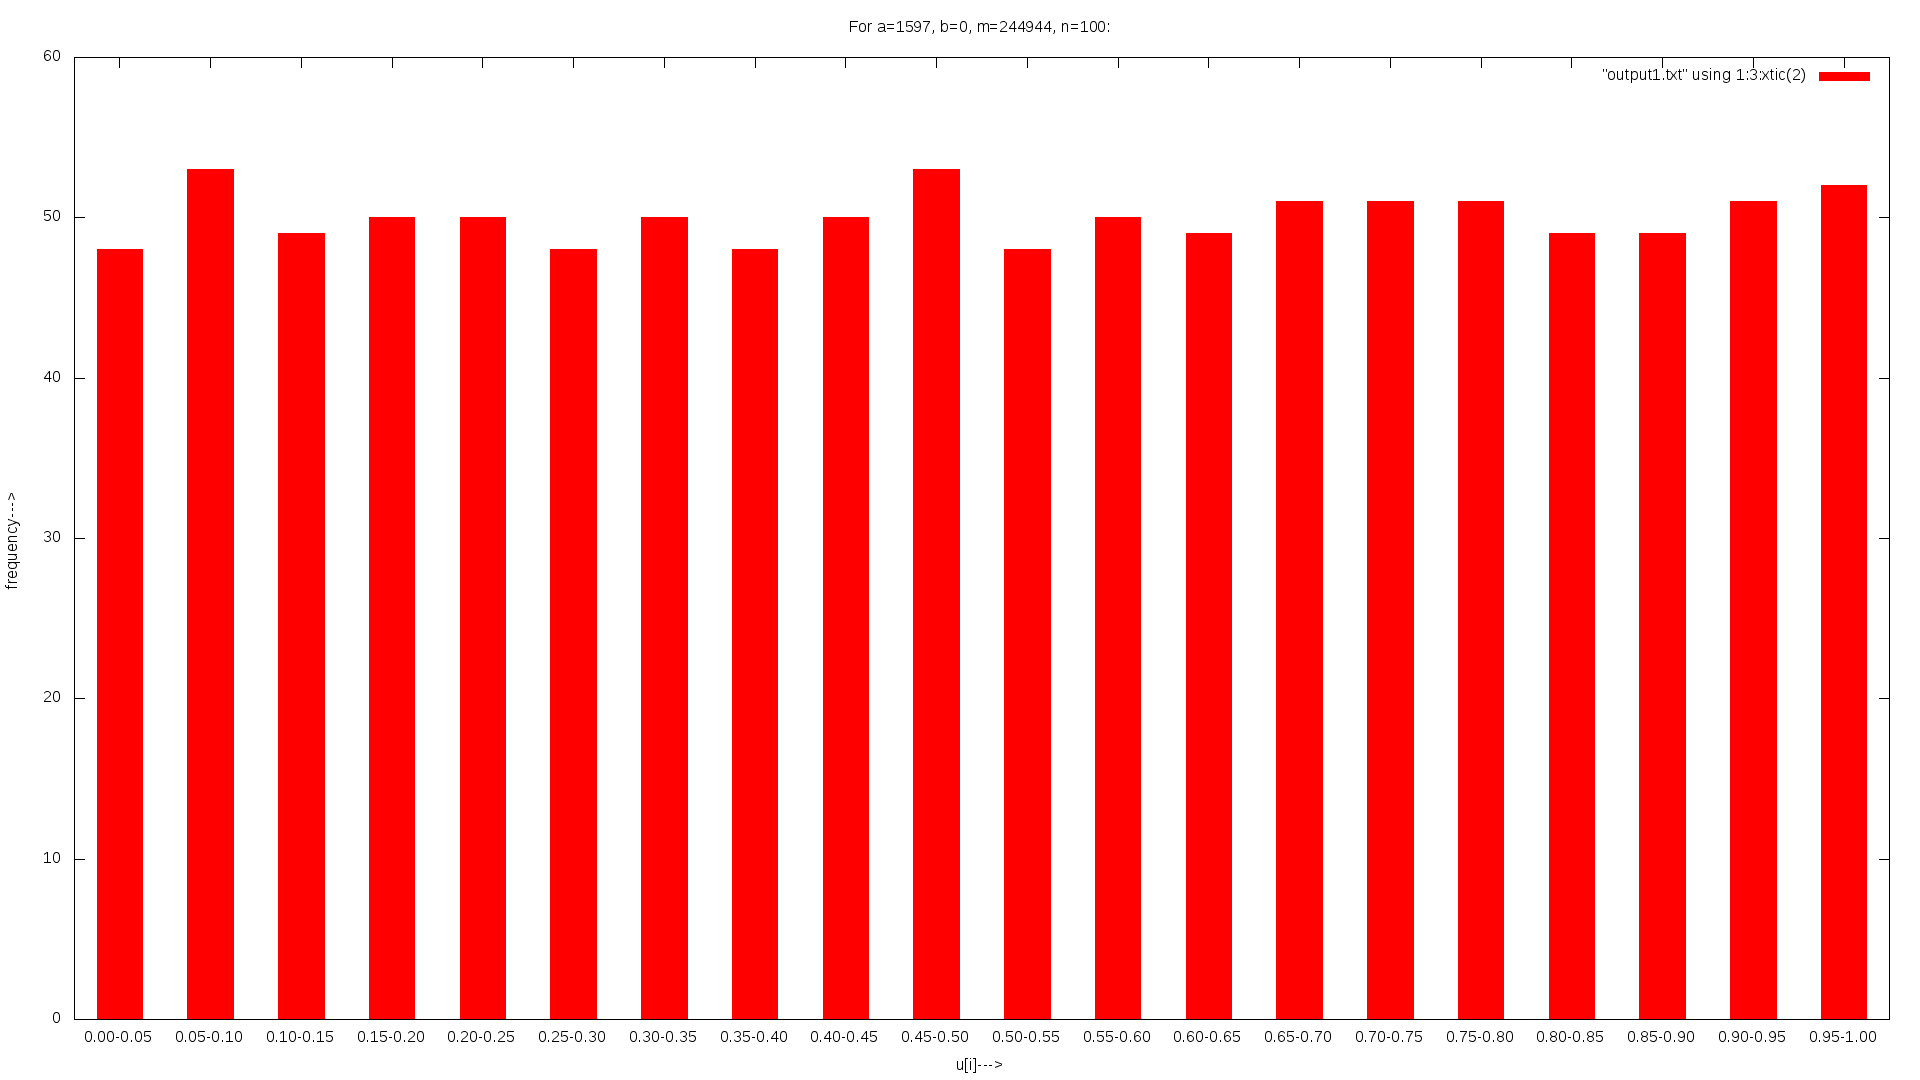
\includegraphics[width=0.5\textwidth]{plot1.png}}\\
	\subfloat[$n=5000$]{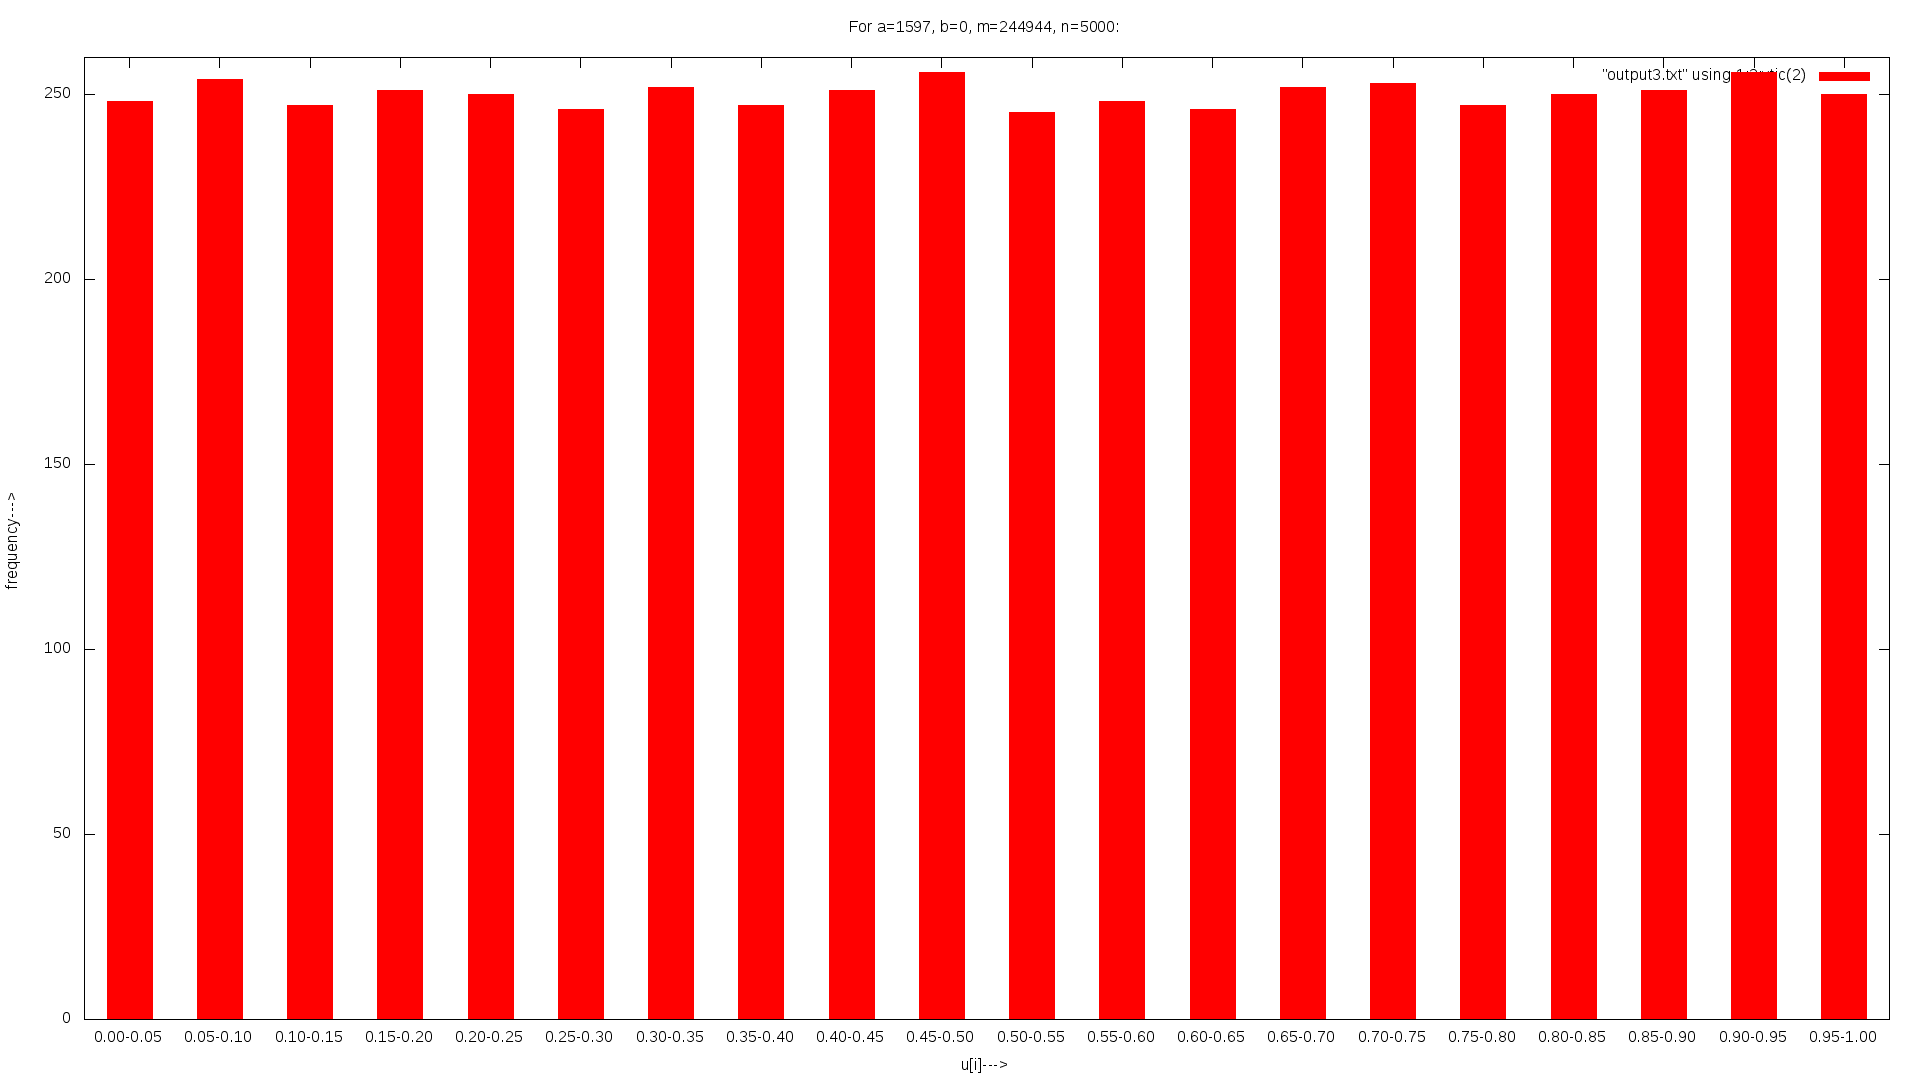
\includegraphics[width=0.5\textwidth]{plot3.png}}
	\subfloat[$n=50000$]{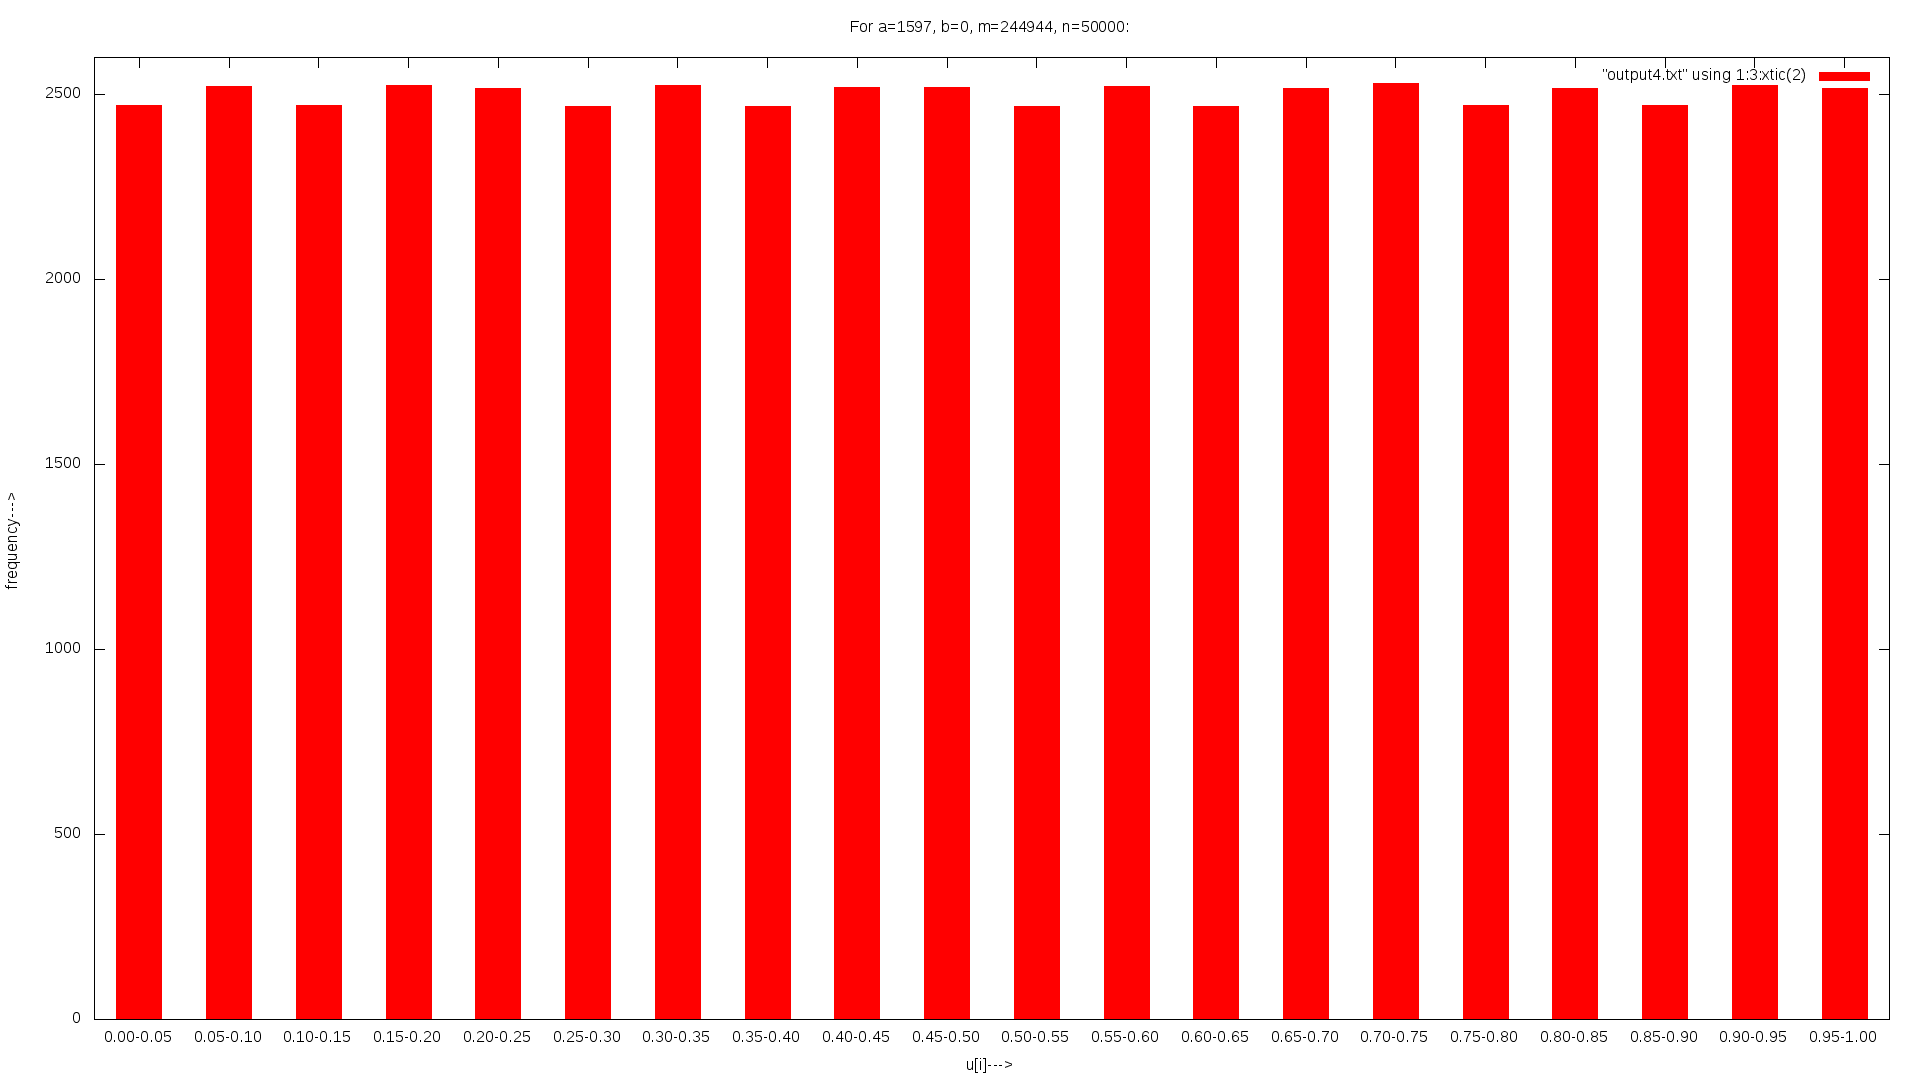
\includegraphics[width=0.5\textwidth]{plot4.png}}\\
	\subfloat[$n=500000$]{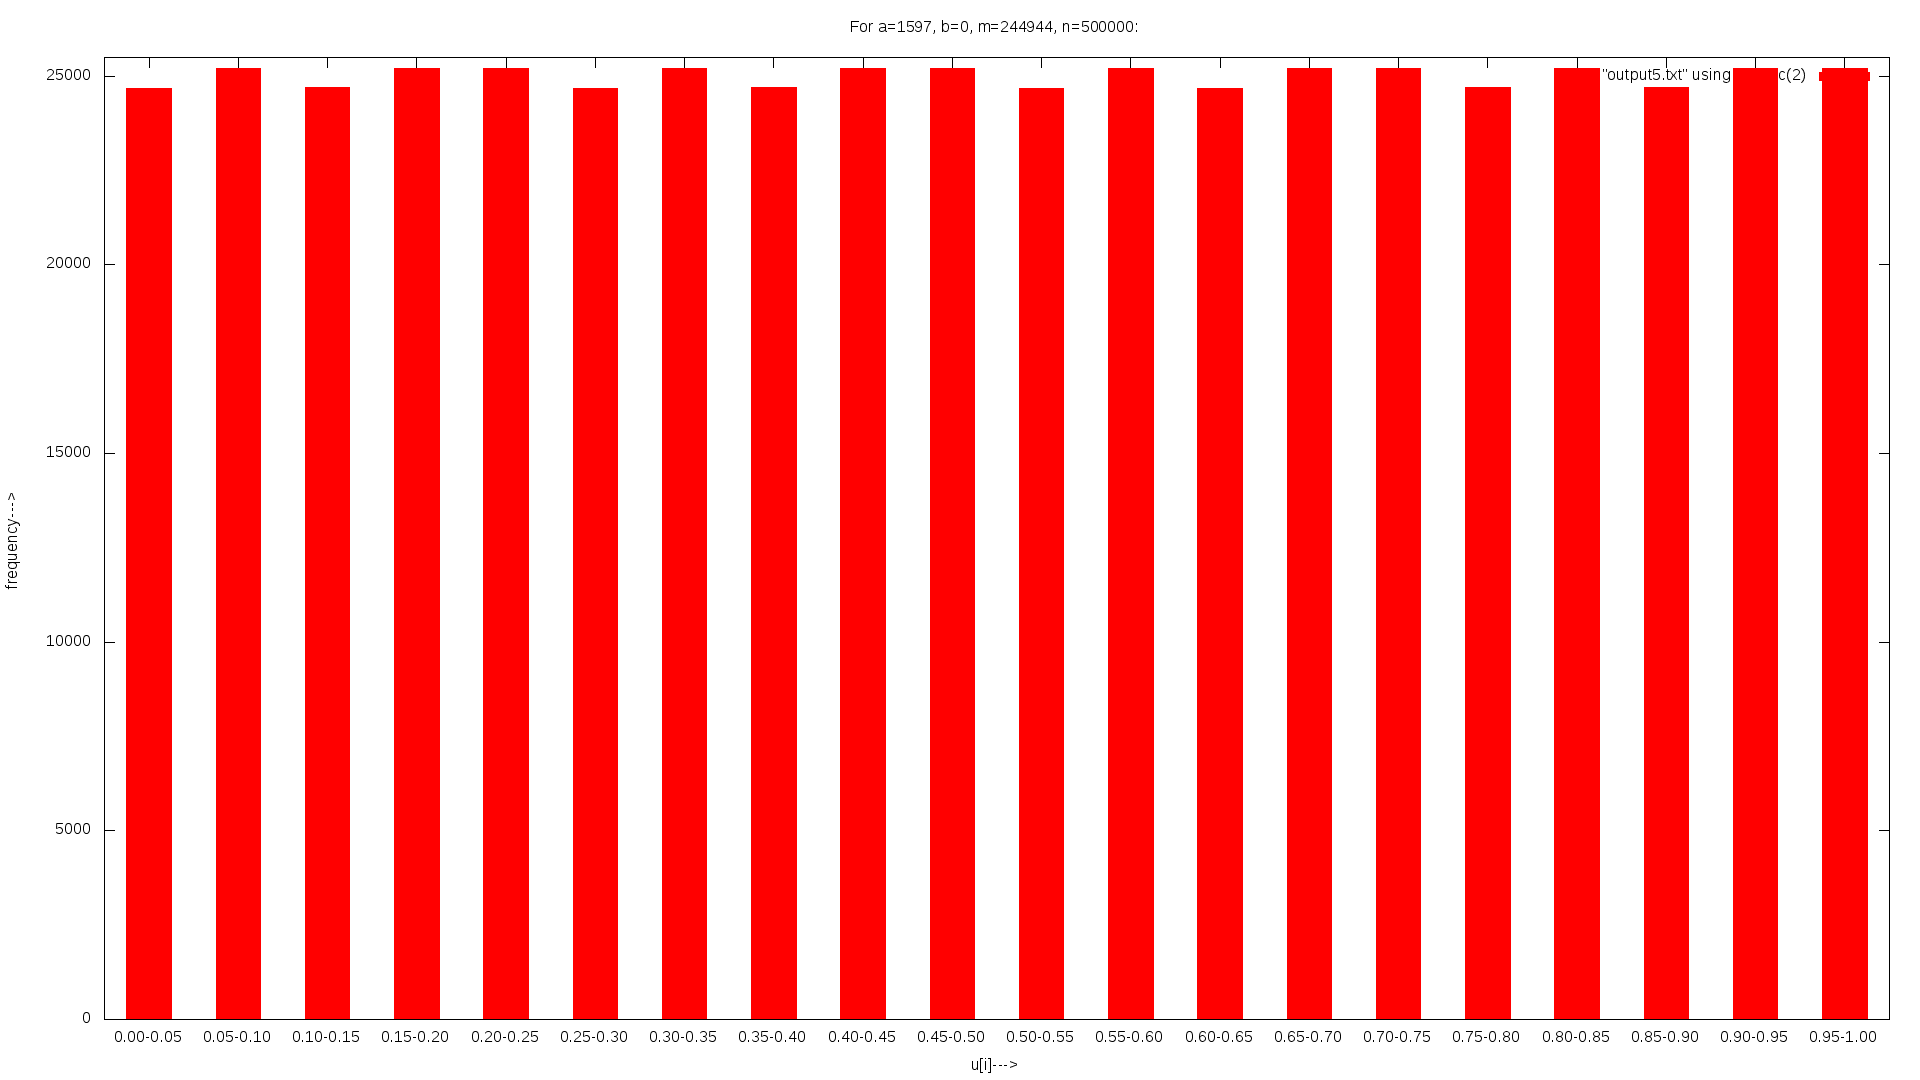
\includegraphics[width=0.5\textwidth]{plot5.png}}
	\caption{Histograms for (a) n = 500, (b) n = 1000 and (c) n = 5000 (d) n = 50000 (e) n = 500000}
\end{figure}
\textbf{Answers:}

\newpage
\Large\textbf{{\underline{Question 3}}}\\\\
Generate a sequence $u_i$ with $a=1229,b=1,m=2048$. Plot a two-dimensional graphthe points $(u_{i-1},u_i)$, i.e. the points $(u_1,u_2),(u_2,u_3),(u_3,u_4),...$ What are your observations?\\\\
\Large\textbf{{\underline{Solution}}}\\\\
C++ Code:
\begin{lstlisting}
#include <iostream>
#include <fstream>

using namespace std;

int main()
{
	ofstream myfile;
	myfile.open("output.txt", ios::app);

	int i,j;
	int a,b,m;
	float x[1000];
	float u[1000];
	a=1229;
	b=1;
	m=2048;
	x[0]=157;
	for(i=0;i<1000;i++)
	{
		x[i+1]=(int((a*x[i])+b))%m;
		u[i+1]=x[i+1]/m;
	}
	u[0]=x[0]/m;
	for(i=0;i<1000;++i)
		myfile<<u[i]<<"		"<<u[i+1]<<"\n";
	myfile.close();
}
\end{lstlisting}
Output:
\begin{lstlisting}
0.0766602		0.21582
0.21582		0.243652
0.243652		0.449219
0.449219		0.090332
0.090332		0.0185547
0.0185547		0.804199
0.804199		0.361328
0.361328		0.0727539
0.0727539		0.415039
0.415039		0.0834961
0.0834961		0.617188
0.617188		0.523926
0.523926		0.905273
0.905273		0.581543
0.581543		0.716797
0.716797		0.943848
0.943848		0.989258
0.989258		0.79834
0.79834		0.160156
0.160156		0.83252
...				...
...				...
...				...
\end{lstlisting}
\textbf{Answers:}

\end{document}
